%%%% utfprpgtex-poster.tex, 2018/09/28
%%%% Copyright (C) 2018 Luiz E. M. Lima (luizeduardomlima@gmail.com)
%%
%% Este arquivo pode ser distribuído e/ou modificado sob as condições da
%% Licença Pública do Projeto LaTeX, tanto a versão 1.3 desta licença ou (à sua
%% opção) qualquer versão posterior.
%% A versão mais recente desta licença está disponível em
%%   http://www.latex-project.org/lppl.txt
%% e a versão 1.3 ou posterior faz parte de todas as distribuições de LaTeX
%% versão 2005/12/01 ou posterior.
%%
%% Este arquivo tem o estado de manutenção da LPPL `mantida'.
%%
%% O mantenedor atual deste arquivo é Luiz E. M. Lima.
%%
%% Este projeto consiste dos arquivos utfprpgtex-poster.sty e
%% utfprpgtex-poster.tex.
%%
%% utfprpgtex-poster.tex é o arquivo principal do modelo LaTeX (não oficial)
%% para produção de poster da Universidade Tecnológica Federal do Paraná
%% (UTFPR). Foi desenvolvido baseado na classe beamer, disponível em
%% <http://ctan.org/pkg/beamer/>, e no pacote beamerposter, disponível em
%% <http://ctan.org/pkg/beamerposter/>.

%% Classe e opções de documento
\documentclass[final]{beamer}

%% Passagem de opções para pacotes
\PassOptionsToPackage{english}{babel}%% Suporte multilíngue
\PassOptionsToPackage{%% Utiliza o modo poster da classe beamer --- Opções
  size = custom,%% Tamanho personalizado
  width = 80,%% Largura em centímetros
  height = 200,% Altura em centímetros
  scale = 1.5,%% Escala de fontes
  debug,%% Modo de depuração
}{beamerposter}

%% Pacotes utilizados
\usepackage{utfprpgtex-poster}%% Estilos do modelo

%% Referências
\AtBeginBibliography{\footnotesize}%% Tamanho de fonte
\addbibresource{utfprpgtex-poster.bib}%% Nome de arquivo

%% Informações do documento
\title{%% Título do poster
  Finite-Time Blowup Construction Research on Navier-Stokes Equations and Euler Equations
}
\subject{Assunto}%% Assunto do poster, e.g.: {Nome do Evento}
\author{%% Autor(es)
  Ben Hou\inst{1}%
}
\institute{%% Instituição(ões) e e-mail(s)
  \inst{1}\utfprname, Beijing, China%
  \par e-mail: \email[1]{hhd16@mails.tsinghua.edu.cn}%
}
\date{}%% Data --- Comente para gerar a data atual

%% Início do documento
\begin{document}

\begin{frame}[t, fragile = singleslide]{}

\begin{columns}[t]%% Cabeçalho

\begin{column}{0.02\textwidth}
\end{column}

\begin{column}{0.18\textwidth}
\flushleft

\includegraphics[width = 0.8\columnwidth]{./Logos/logo-event}%% Logomarca superior-esquerdo
%\vspace*{\baselineskip}
%
\includegraphics[width = 0.8\columnwidth]{./Logos/logo-org}%% Logomarca inferior-esquerdo
\end{column}

\begin{column}{0.6\textwidth}
\titlepage
\end{column}

\begin{column}{0.18\textwidth}
\flushright

\includegraphics[width = 0.8\columnwidth]{./Logos/logo-tsinghua}%% Logomarca superior-direito
%\vspace*{\baselineskip}
%
\includegraphics[width = 0.8\columnwidth]{./Logos/logo-inst-ext}%% Logomarca inferior-direito
\end{column}

\begin{column}{0.02\textwidth}
\end{column}

\end{columns}

\begin{columns}[t]

\begin{column}{0.45\textwidth}

\begin{block}{INTRODUÇÃO}
\begin{itemize}
\item Este poster foi desenvolvido com base na classe \LaTeX/Beamer, disponível em <\url{http://www.ctan.org/pkg/beamer/}>, usando o pacote \LaTeX\ ``beamerposter'', disponível em <\url{http://ctan.org/pkg/beamerposter/}>.
\item Exemplos de referências podem ser observados nas citações:
\begin{itemize}
\item Implícita: ... \cite{Lamport1994,VanEkenstein1997}.
\item Explícita: Segundo \textcite{Wizentier1992},...
\end{itemize}
\item Citações e referências podem ser inseridas neste documento usando os comandos do pacote \LaTeX\ ``biblatex'', disponível em <\url{http://ctan.org/pkg/biblatex/}>.
\item Os dados de cada referência podem ser obtidos de um arquivo ``bibtex'' (*.bib), geralmente na própria página de \textit{download} da referência (artigos, livros, etc.), ou no Google Acadêmico, etc.
\item Para gerar ou editar entradas de arquivos ``bibtex'' (*.bib) pode-se utilizar a ferramenta ``Bibtex Editor'', disponível em <\url{http://truben.no/latex/bibtex/}>, ou ``ZoteroBib'', disponível em <\url{http://zbib.org/}>, dentre outras.
\end{itemize}
\end{block}

\begin{block}{REVISÃO DA LITERATURA}
Exemplo de lista de itens numerada:
\begin{enumerate}
\item Item numerado 1.
\item Item numerado 2.
\item Item numerado 3.
\end{enumerate}
Uma equação como $y = a x^2 + b x + c$ pode ser inserida ao longo do texto de um parágrafo usando o ambiente \LaTeX\ ``math'' (\verb|$...$|). Por outro lado, a seguinte equação é um exemplo de equação não numerada inserida numa linha em separado usando o ambiente \LaTeX\ ``displaymath'' (\verb|\[...\]|).
\[
\frac{\mathrm{d}y}{\mathrm{d}x} = \gamma \ \mathrm{sen} x
\]
A Equação~\eqref{eq:fx} é um exemplo de equação inserida usando o ambiente \LaTeX\ ``equation'' e numerada automaticamente.
\begin{equation}\label{eq:fx}
f(x) = \frac{1}{\alpha} \int^L_0 \left(\frac{x^2}{2} - \frac{x^3}{3}\right) \mathrm{d}x
\end{equation}
Para gerar ou editar equações em \LaTeX\ pode-se utilizar a ferramenta ``Formula Sheet'', disponível em <\url{http://formulasheet.com/}>, dentre outras.
\end{block}

\end{column}

\begin{column}{0.45\textwidth}

\begin{block}{MATERIAL E MÉTODOS}
A Figura~\ref{fig:campuspontagrossa} é um exemplo de figura inserida usando o ambiente \LaTeX\ ``figure'' e numerada automaticamente.
\begin{figure}[!htb]
\centering
\caption{Exemplo de legenda de figura.}
\label{fig:campuspontagrossa}
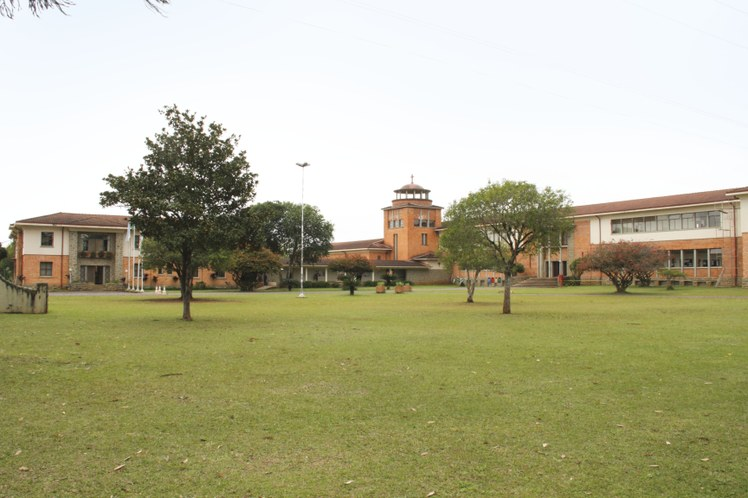
\includegraphics[width = 0.675\columnwidth]{./Figuras/campuspontagrossa}
\source{\textcite{UTFPR2018}.}
\end{figure}
A Tabela~\ref{tab:Ldimensoes} é um exemplo de tabela inserida usando o ambiente \LaTeX\ ``table'' e numerada automaticamente.
\begin{table}[!htb]
\centering\small
\caption{Exemplo de legenda de tabela.}
\label{tab:Ldimensoes}
\begin{tabular*}{\columnwidth}{@{\extracolsep{\fill}}llll}
\hline
$L$   & $L^2$     & $L^3$     & $L^4$     \\
{[m]} & {[m$^2$]} & {[m$^3$]} & {[m$^4$]} \\ \hline
1     & 1         & 1         & 1         \\
2     & 4         & 8         & 16        \\
3     & 9         & 27        & 81        \\
4     & 16        & 64        & 256       \\
5     & 25        & 125       & 625       \\ \hline
\end{tabular*}
\source{Autoria própria.}
\end{table}
Para gerar ou editar tabelas em \LaTeX\ pode-se utilizar a ferramenta ``Tables Generator'', disponível em <\url{http://www.tablesgenerator.com/}>, dentre outras.\par
Informações e dicas sobre \TeX/\LaTeX\ podem ser obtidas em:
\begin{itemize}
\item \LaTeX\ Project: <\url{http://www.latex-project.org/}>.
\item Comprehensive \TeX\ Archive Network (CTAN): <\url{http://www.ctan.org/}>.
\item \TeX\ Users Group (TUG): <\url{http://www.tug.org/}>.
\item \LaTeX\ - Wikibooks: <\url{http://en.wikibooks.org/wiki/LaTeX/}>.
\item \TeX\ - \LaTeX\ Stack Exchange: <\url{http://tex.stackexchange.com/}>.
\end{itemize}
\end{block}

\end{column}

\end{columns}

\begin{columns}[t]

\begin{column}{0.945\textwidth}

\begin{block}{RESULTADOS E DISCUSSÃO}
As Figuras~\ref{fig:graficoxy1}, \ref{fig:graficoxy2} e \ref{fig:graficoxy3} são mais exemplos de figuras inseridas usando o ambiente \LaTeX\ ``figure'' e dispostas em três colunas.
\begin{column}[T]{0.33\textwidth}
\begin{figure}[!htb]
\centering
\caption{Exemplo de legenda de figura.}
\label{fig:graficoxy1}
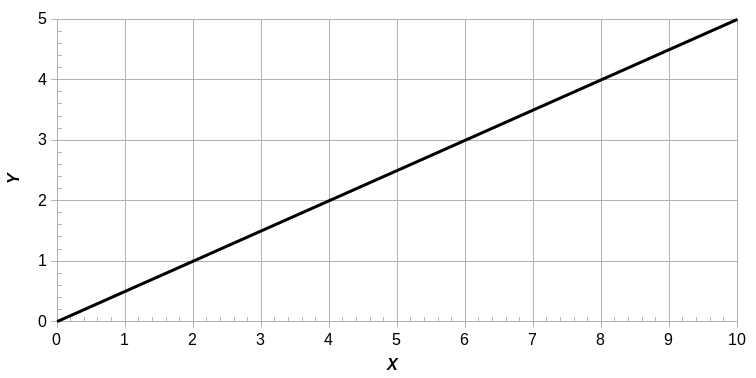
\includegraphics[width = 0.75\columnwidth]{./Figuras/graficoxy}
\source{Autoria própria.}
\end{figure}
\end{column}
{\color{tsinghua}\vrule width 1.5pt}
\begin{column}[T]{0.33\textwidth}
\begin{figure}[!htb]
\centering
\caption{Exemplo de legenda de figura.}
\label{fig:graficoxy2}
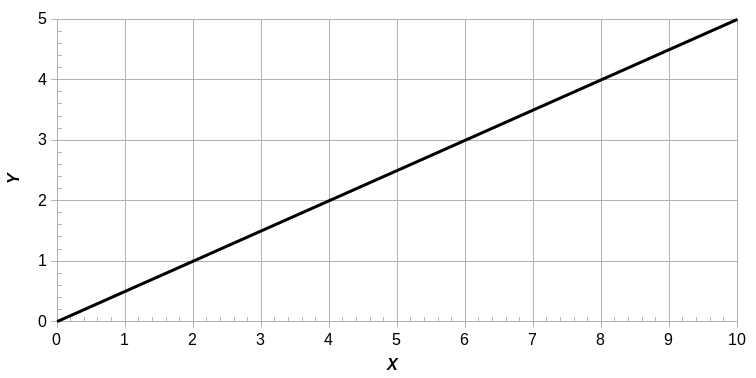
\includegraphics[width = 0.75\columnwidth]{./Figuras/graficoxy}
\source{Autoria própria.}
\end{figure}
\end{column}
{\color{tsinghua}\vrule width 1.5pt}
\begin{column}[T]{0.33\textwidth}
\begin{figure}[!htb]
\centering
\caption{Exemplo de legenda de figura.}
\label{fig:graficoxy3}
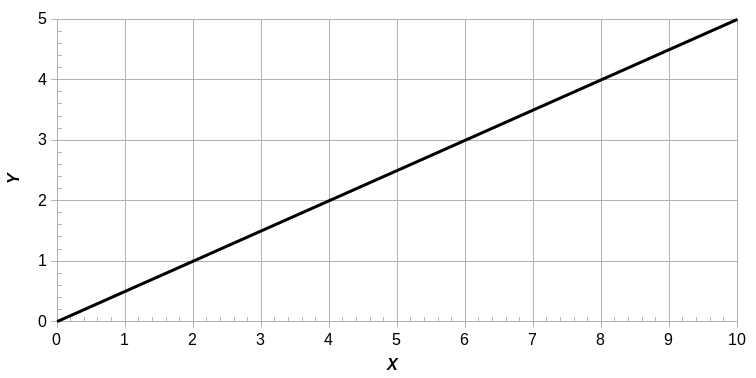
\includegraphics[width = 0.75\columnwidth]{./Figuras/graficoxy}
\source{Autoria própria.}
\end{figure}
\end{column}
\end{block}

\end{column}

\end{columns}

\begin{columns}[t]

\begin{column}{0.45\textwidth}

\begin{block}{CONCLUSÕES}
\begin{itemize}
\item Conclusão 1.
\item Conclusão 2.
\item Conclusão 3.
\item Conclusão 4.
\item Conclusão 5.
\end{itemize}
\end{block}

\begin{block}{AGRADECIMENTOS}
\footnotesize
Pelo apoio recebido para o desenvolvimento deste trabalho e a participação neste evento:
\vfill

\includegraphics[height = 30mm]{./Logos/logo-capes}
\hspace*{5mm}

\includegraphics[height = 30mm]{./Logos/logo-cnpq}
\hspace*{5mm}

\includegraphics[height = 30mm]{./Logos/logo-fa}
\hspace*{5mm}

\includegraphics[height = 30mm]{./Logos/logo-utfpr}
\end{block}

\end{column}

\begin{column}{0.45\textwidth}

\begin{block}{REFERÊNCIAS}
\printbibliography[heading = none]
\end{block}

\end{column}

\end{columns}

\begin{columns}[t]

\begin{column}{0.945\textwidth}
\vfill
\begin{tiny}
\textbf{Declaração de Responsabilidade:} O(s) autor(es) é(são) o(s) único(s) responsável(eis) pelo material impresso contido neste documento.
\end{tiny}
\end{column}

\end{columns}

\end{frame}

%% Fim do documento
\end{document}
